\documentclass[a4paper,12pt]{paper}

\usepackage{mycommands}

% Worked-example layout: boxed problem statement followed by a solution.
\newcounter{example}
\renewenvironment{example}[1]{%  % the paper class already defines "example"
  \refstepcounter{example}%
  \begin{mdframed}[linewidth=1pt,innertopmargin=6pt,innerbottommargin=6pt]%
  \noindent\textbf{Example \theexample: #1.}\ }{%
  \end{mdframed}}
\newenvironment{solution}{\par\noindent\textbf{Solution.}\ }{\par\medskip}

\title{Worked examples for Lecture 16: Ray theory}
\author{David Al-Attar \\ Michaelmas Term, \the\year}

\begin{document}

\maketitle

\noindent These examples accompany Lecture~16. They are intended as practice in the concrete
calculations that underlie the lecture, and are less demanding than the questions on the
problem sets. Numerical results were checked with the scripts in the \texttt{python}
directory.

\begin{example}{The isotropic eikonal equation and a linear velocity gradient}
(a) Show that in an isotropic medium with P-wave speed $\alpha(\mathbf{x})$ the eikonal equation
for the P-wave sheet of the local slowness surface reduces to $\|\nabla T\|=1/\alpha$, and that the
corresponding ray Hamiltonian is $H(\mathbf{x},\mathbf{p})=\frac{1}{2}\alpha(\mathbf{x})^{2}\|\mathbf{p}\|^{2}$.

\noindent (b) Consider a two-dimensional model with horizontal coordinate $x$, depth $z$ measured
positively downwards, and P-wave speed $\alpha(z)=\alpha_{0}+gz$ with $\alpha_{0}>0$ and $g>0$.
A ray leaves the origin with take-off angle $\theta_{0}$ measured from the downward vertical.
Solve Hamilton's equations for this ray. Show that the horizontal slowness
$p_{x}=\sin\theta_{0}/\alpha_{0}$ is conserved, that the ray is a circular arc of radius
$R=1/(gp_{x})$ centred at the depth $z=-\alpha_{0}/g$, and that the travel time along the ray is
\begin{equation*}
T=\frac{1}{g}\ln\left[\frac{\tan(\theta/2)}{\tan(\theta_{0}/2)}\right],
\end{equation*}
where $\theta$ is the angle the ray makes with the downward vertical at the point in question.

\noindent (c) Find the horizontal distance $X$ at which the ray returns to the surface $z=0$ and the
travel time $T(X)$, and evaluate both for $\alpha_{0}=5\,\mathrm{km\,s^{-1}}$, $g=0.05\,\mathrm{s^{-1}}$
and $\theta_{0}=30^{\circ}$.
\end{example}

\begin{solution}
(a) In an isotropic medium the elastic tensor is
$A_{ijkl}=\lambda\delta_{ij}\delta_{kl}+\mu(\delta_{ik}\delta_{jl}+\delta_{il}\delta_{jk})$, and so the
local Christoffel operator defined in the lecture takes the form
\begin{equation}
\Gamma_{ik}(\mathbf{x},\mathbf{p})=\frac{1}{\rho}A_{ijkl}p_{j}p_{l}
=\alpha^{2}p_{i}p_{k}+\beta^{2}\left(\|\mathbf{p}\|^{2}\delta_{ik}-p_{i}p_{k}\right),
\label{eq:1}
\end{equation}
with $\alpha^{2}=(\lambda+2\mu)/\rho$ and $\beta^{2}=\mu/\rho$, exactly as for plane waves in
Lecture~15 but with $\rho$, $\lambda$ and $\mu$ now functions of $\mathbf{x}$. The two terms are,
respectively, $\|\mathbf{p}\|^{2}$ times the projections parallel and orthogonal to
$\hat{\mathbf{p}}$, so the eigenvalues of $\bm{\Gamma}$ are $\alpha^{2}\|\mathbf{p}\|^{2}$, with
eigenvector $\hat{\mathbf{p}}$, and $\beta^{2}\|\mathbf{p}\|^{2}$, with the two-dimensional
eigenspace orthogonal to $\hat{\mathbf{p}}$. The eikonal equation
$\det(\bm{\Gamma}-\mathbf{I})=0$ therefore factorises as
\begin{equation}
\left(\alpha^{2}\|\mathbf{p}\|^{2}-1\right)\left(\beta^{2}\|\mathbf{p}\|^{2}-1\right)^{2}=0,
\label{eq:2}
\end{equation}
which is the lecture's general factorised form with the local phase speeds
$c_{1}=\alpha$ and $c_{2}=c_{3}=\beta$ independent of the direction $\hat{\mathbf{p}}$. Selecting
the P-wave sheet and recalling that $\mathbf{p}=\nabla T$, the reduced eikonal equation is
\begin{equation}
\alpha(\mathbf{x})^{2}\|\nabla T(\mathbf{x})\|^{2}=1,\quad\text{i.e.}\quad
\|\nabla T\|=\frac{1}{\alpha},
\label{eq:3}
\end{equation}
and the ray Hamiltonian $H=\frac{1}{2}\|\mathbf{p}\|^{2}c_{1}^{2}$ of the lecture becomes
\begin{equation}
H(\mathbf{x},\mathbf{p})=\frac{1}{2}\alpha(\mathbf{x})^{2}\|\mathbf{p}\|^{2},
\label{eq:4}
\end{equation}
with the eikonal equation being $H[\mathbf{x},\nabla T(\mathbf{x})]=\frac{1}{2}$. The polarisation
$\hat{\mathbf{a}}^{0}=\hat{\mathbf{p}}$ is, as for plane waves, along the local direction of
propagation.

\noindent (b) We work in the $(x,z)$-plane, with $\mathbf{x}=(x,z)$ and $\mathbf{p}=(p_{x},p_{z})$,
and the sign conventions stated in the question: $z$ increases downwards, so that $\alpha$
increases with depth, and a ray travelling straight down has $\theta=0$. The initial point in phase
space is $\mathbf{x}^{0}=(0,0)$ together with
\begin{equation}
\mathbf{p}^{0}=\frac{1}{\alpha_{0}}(\sin\theta_{0},\cos\theta_{0}),
\label{eq:5}
\end{equation}
which has $\|\mathbf{p}^{0}\|=1/\alpha_{0}$ and so satisfies $H=\frac{1}{2}$ as required. From
eq.~(\ref{eq:4}), $\partial H/\partial p_{i}=\alpha^{2}p_{i}$ and
$\partial H/\partial x_{i}=\alpha\|\mathbf{p}\|^{2}\,\partial\alpha/\partial x_{i}$, and since
$\alpha$ depends only on $z$ with $\ddns\alpha/\ddns z=g$, Hamilton's canonical equations read
\begin{equation}
\frac{\ddns x}{\ddns\sigma}=\alpha^{2}p_{x},\quad
\frac{\ddns z}{\ddns\sigma}=\alpha^{2}p_{z},\quad
\frac{\ddns p_{x}}{\ddns\sigma}=0,\quad
\frac{\ddns p_{z}}{\ddns\sigma}=-\|\mathbf{p}\|^{2}\alpha g=-\frac{g}{\alpha},
\label{eq:6}
\end{equation}
where in the last equation we have used the conservation of the Hamiltonian,
$\alpha^{2}\|\mathbf{p}\|^{2}=1$, along the solution. The third equation shows at once that the
horizontal slowness is conserved,
\begin{equation}
p_{x}=\frac{\sin\theta_{0}}{\alpha_{0}}\equiv p,
\label{eq:7}
\end{equation}
which is the conserved quantity associated with the translational symmetry of the model in $x$; it
is often called the ray parameter. Because $\|\mathbf{p}\|=1/\alpha$ everywhere along the ray, we
can introduce an angle $\theta(\sigma)$ through
\begin{equation}
p_{x}=\frac{\sin\theta}{\alpha},\quad p_{z}=\frac{\cos\theta}{\alpha},
\label{eq:8}
\end{equation}
with $\theta(0)=\theta_{0}$. The first two equations in eq.~(\ref{eq:6}) then give
$\ddns\mathbf{x}/\ddns\sigma=\alpha(\sin\theta,\cos\theta)$, so $\theta$ is precisely the angle
between the ray and the downward vertical, and $\ddns s/\ddns\sigma=\alpha$ for the arc length
$s$ along the ray. Combining eqs.~(\ref{eq:7}) and (\ref{eq:8}) we obtain Snell's law for this
model,
\begin{equation}
\frac{\sin\theta}{\alpha(z)}=p,
\label{eq:9}
\end{equation}
so that $\theta$ increases with depth: the ray turns away from the vertical as it enters faster
material. Differentiating eq.~(\ref{eq:9}) with respect to $\sigma$ and using
$\ddns z/\ddns\sigma=\alpha\cos\theta$ gives
$\cos\theta\,\ddns\theta/\ddns\sigma=pg\alpha\cos\theta$, and hence
\begin{equation}
\frac{\ddns\theta}{\ddns\sigma}=pg\alpha=g\sin\theta.
\label{eq:10}
\end{equation}
It is now simplest to use $\theta$ rather than $\sigma$ as the parameter along the ray. Dividing
$\ddns x/\ddns\sigma=\alpha\sin\theta$ and $\ddns z/\ddns\sigma=\alpha\cos\theta$ by
eq.~(\ref{eq:10}), and writing $R=1/(gp)$, we find
\begin{equation}
\frac{\ddns x}{\ddns\theta}=\frac{\alpha}{g}=R\sin\theta,\quad
\frac{\ddns z}{\ddns\theta}=\frac{\alpha\cos\theta}{g\sin\theta}=R\cos\theta,
\label{eq:11}
\end{equation}
where we have used $\alpha=\sin\theta/p$ from eq.~(\ref{eq:9}). Integrating from
$\theta_{0}$, where the ray is at the origin,
\begin{equation}
x=R(\cos\theta_{0}-\cos\theta),\quad z=R(\sin\theta-\sin\theta_{0}),
\label{eq:12}
\end{equation}
and therefore
\begin{equation}
(x-R\cos\theta_{0})^{2}+(z+R\sin\theta_{0})^{2}=R^{2}.
\label{eq:13}
\end{equation}
The ray is a circle of radius
\begin{equation}
R=\frac{1}{gp}=\frac{\alpha_{0}}{g\sin\theta_{0}},
\label{eq:14}
\end{equation}
whose centre lies at horizontal position $R\cos\theta_{0}$ and at the depth
$-R\sin\theta_{0}=-\alpha_{0}/g$. This depth is the same for all take-off angles: it is the
height above the surface at which the linear velocity profile would extrapolate to zero. Note also
that eq.~(\ref{eq:11}) gives $\ddns s/\ddns\theta=R$, so the curvature $\ddns\theta/\ddns s=1/R$
is indeed constant along the ray.

For the travel time we use the lecture's result that the generating parameter is the travel time,
$T[\mathbf{x}(\sigma)]=\sigma$, together with eq.~(\ref{eq:10}):
\begin{equation}
T=\int_{0}^{\sigma}\dd\sigma'=\int_{\theta_{0}}^{\theta}\frac{\dd\theta'}{g\sin\theta'}
=\frac{1}{g}\ln\left[\frac{\tan(\theta/2)}{\tan(\theta_{0}/2)}\right],
\label{eq:15}
\end{equation}
where we have used $\frac{\ddns}{\ddns\theta}\ln\tan(\theta/2)=1/\sin\theta$. The same result follows
from $\dd T=\dd s/\alpha=R\,\dd\theta/\alpha$ and eq.~(\ref{eq:9}).

\noindent (c) The ray is horizontal, $\theta=\pi/2$, at its turning point, which from eq.~(\ref{eq:12})
lies at the depth
\begin{equation}
z_{t}=R(1-\sin\theta_{0})=\frac{\alpha_{0}}{g}\left(\frac{1}{\sin\theta_{0}}-1\right),
\label{eq:16}
\end{equation}
and by the symmetry of the circle it returns to $z=0$ when $\theta=\pi-\theta_{0}$, at the distance
\begin{equation}
X=2R\cos\theta_{0}=\frac{2\alpha_{0}}{g}\cot\theta_{0}.
\label{eq:17}
\end{equation}
Setting $\theta=\pi-\theta_{0}$ in eq.~(\ref{eq:15}) and using $\tan[(\pi-\theta_{0})/2]=\cot(\theta_{0}/2)$,
\begin{equation}
T(X)=\frac{2}{g}\ln\cot\frac{\theta_{0}}{2}=\frac{2}{g}\,\mathrm{arcsinh}\left(\frac{gX}{2\alpha_{0}}\right),
\label{eq:18}
\end{equation}
where the second form follows from $\cot(\theta_{0}/2)=\cot\theta_{0}+\sqrt{1+\cot^{2}\theta_{0}}$ and
$\mathrm{arcsinh}\,u=\ln(u+\sqrt{1+u^{2}})$, with $u=\cot\theta_{0}=gX/(2\alpha_{0})$ from
eq.~(\ref{eq:17}). Eq.~(\ref{eq:18}) is the travel-time curve for this model. For small $X$ it reduces
to $T\approx X/\alpha_{0}$, while for large $X$ the travel time grows only logarithmically because the
ray spends most of its time in fast material at depth. For the given numbers,
$p=0.1\,\mathrm{s\,km^{-1}}$, $R=200\,\mathrm{km}$, the centre of the circle lies at
$(173.2,-100)\,\mathrm{km}$, the turning depth is $z_{t}=100\,\mathrm{km}$, the ray returns to the
surface at $X=346.4\,\mathrm{km}$, and $T(X)=40\ln\cot 15^{\circ}=52.68\,\mathrm{s}$. This is
considerably less than the $69.28\,\mathrm{s}$ that would be taken along the straight line at speed
$\alpha_{0}$. Integrating Hamilton's equations in eq.~(\ref{eq:6}) numerically with
\texttt{scipy.integrate.solve\_ivp} reproduces the circle to $10^{-7}\,\mathrm{km}$ and the travel
time to $10^{-8}\,\mathrm{s}$. Fig.~\ref{fig:1} shows the resulting fan of rays.

\begin{figure}[ht]
\centering
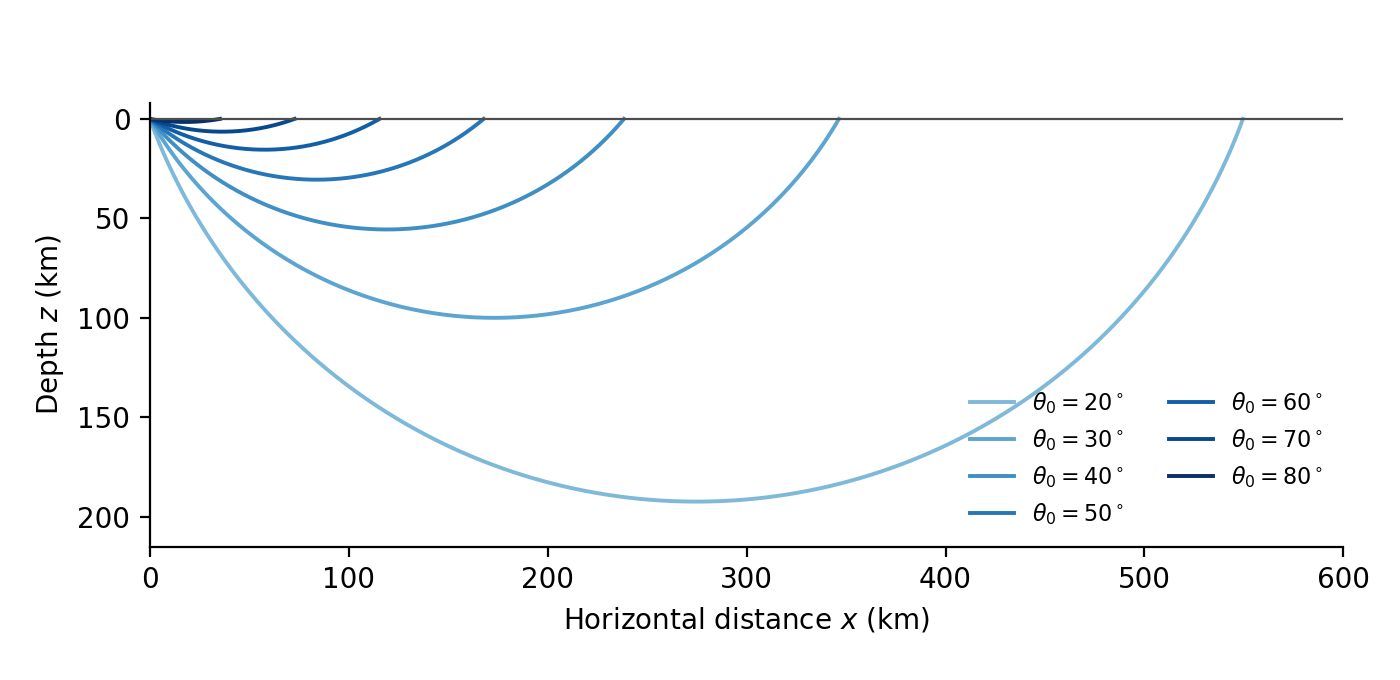
\includegraphics[width=0.7\textwidth]{figures_ex/ex5_rays.png}
\caption{Fan of rays leaving the origin in the model $\alpha(z)=\alpha_{0}+gz$ with
$\alpha_{0}=5\,\mathrm{km\,s^{-1}}$ and $g=0.05\,\mathrm{s^{-1}}$, for take-off angles between
$20^{\circ}$ and $80^{\circ}$. Each ray is a circular arc centred at the depth $-\alpha_{0}/g=-100\,\mathrm{km}$.}
\label{fig:1}
\end{figure}

This example is the simplest illustration of how a velocity that increases with depth returns rays
to the surface, which is the mechanism that makes body-wave seismology possible; the spherical
analogue is developed in Lecture~17.
\end{solution}

\begin{example}{From Hamilton's equations to the ray equation}
For the isotropic P-wave Hamiltonian $H(\mathbf{x},\mathbf{p})=\frac{1}{2}\alpha(\mathbf{x})^{2}\|\mathbf{p}\|^{2}$
write down Hamilton's equations. Show that the arc length $s$ along a ray satisfies
$\ddns s/\ddns\sigma=\alpha$, and hence that rays satisfy the ray equation
\begin{equation*}
\frac{\ddns}{\ddns s}\left(\frac{1}{\alpha}\frac{\ddns\mathbf{x}}{\ddns s}\right)=\nabla\left(\frac{1}{\alpha}\right).
\end{equation*}
Deduce that rays are straight lines when $\alpha$ is constant, and show that in general a ray has
curvature $\kappa=\|\hat{\mathbf{t}}\times\nabla\ln\alpha\|$, where $\hat{\mathbf{t}}$ is the unit
tangent, and bends towards regions of lower wave speed. Check the result against Example~1.
\end{example}

\begin{solution}
The partial derivatives of the Hamiltonian are $\partial H/\partial p_{i}=\alpha^{2}p_{i}$
and $\partial H/\partial x_{i}=\alpha\|\mathbf{p}\|^{2}\,\partial\alpha/\partial x_{i}$, and so
Hamilton's equations are
\begin{equation}
\frac{\ddns\mathbf{x}}{\ddns\sigma}=\alpha^{2}\mathbf{p},\quad
\frac{\ddns\mathbf{p}}{\ddns\sigma}=-\|\mathbf{p}\|^{2}\alpha\nabla\alpha.
\label{eq:19}
\end{equation}
Along a solution the Hamiltonian is conserved and equal to $\frac{1}{2}$, so $\|\mathbf{p}\|=1/\alpha$,
and the equations simplify to
\begin{equation}
\frac{\ddns\mathbf{x}}{\ddns\sigma}=\alpha\hat{\mathbf{p}},\quad
\frac{\ddns\mathbf{p}}{\ddns\sigma}=-\frac{\nabla\alpha}{\alpha}=-\nabla\ln\alpha.
\label{eq:20}
\end{equation}
The first of these shows that the ray is everywhere tangent to the local slowness vector, and that
\begin{equation}
\frac{\ddns s}{\ddns\sigma}=\left\|\frac{\ddns\mathbf{x}}{\ddns\sigma}\right\|=\alpha,
\label{eq:21}
\end{equation}
which is just the statement $\dd T=\dd s/\alpha$ that the travel time accumulates at the local
slowness. The unit tangent is therefore
\begin{equation}
\hat{\mathbf{t}}=\frac{\ddns\mathbf{x}}{\ddns s}=\frac{1}{\alpha}\frac{\ddns\mathbf{x}}{\ddns\sigma}=\hat{\mathbf{p}},
\quad\text{so that}\quad \mathbf{p}=\frac{1}{\alpha}\frac{\ddns\mathbf{x}}{\ddns s}.
\label{eq:22}
\end{equation}
Differentiating this expression with respect to $s$ and using eqs.~(\ref{eq:20}) and (\ref{eq:21}),
\begin{equation}
\frac{\ddns}{\ddns s}\left(\frac{1}{\alpha}\frac{\ddns\mathbf{x}}{\ddns s}\right)
=\frac{\ddns\mathbf{p}}{\ddns s}=\frac{1}{\alpha}\frac{\ddns\mathbf{p}}{\ddns\sigma}
=-\frac{\nabla\alpha}{\alpha^{2}}=\nabla\left(\frac{1}{\alpha}\right),
\label{eq:23}
\end{equation}
which is the ray equation. It is a second-order equation for the ray path alone, with the slowness
vector eliminated; it is also the Euler--Lagrange equation for Fermat's principle of stationary
travel time $\int\dd s/\alpha$, though we do not need that here. If $\alpha$ is constant the
right hand side vanishes and $\ddns^{2}\mathbf{x}/\ddns s^{2}=\mathbf{0}$, so rays are straight
lines, as they must be if the theory is to reproduce plane waves in a homogeneous body.

To find the curvature we expand the left hand side of eq.~(\ref{eq:23}), using the chain
rule in the form $\ddns(1/\alpha)/\ddns s=\hat{\mathbf{t}}\cdot\nabla(1/\alpha)$, which gives
\begin{equation}
\frac{1}{\alpha}\frac{\ddns\hat{\mathbf{t}}}{\ddns s}+\hat{\mathbf{t}}\left[\hat{\mathbf{t}}\cdot\nabla\left(\frac{1}{\alpha}\right)\right]
=\nabla\left(\frac{1}{\alpha}\right).
\label{eq:24}
\end{equation}
Multiplying by $\alpha$ and using $\alpha\nabla(1/\alpha)=-\nabla\ln\alpha$,
\begin{equation}
\frac{\ddns\hat{\mathbf{t}}}{\ddns s}=-\left[\nabla\ln\alpha-\hat{\mathbf{t}}(\hat{\mathbf{t}}\cdot\nabla\ln\alpha)\right]
=-(\nabla\ln\alpha)_{\perp},
\label{eq:25}
\end{equation}
where $(\nabla\ln\alpha)_{\perp}$ denotes the component of $\nabla\ln\alpha$ orthogonal to the ray.
By the Frenet formula $\ddns\hat{\mathbf{t}}/\ddns s=\kappa\hat{\mathbf{n}}$, with $\kappa\ge0$ the
curvature and $\hat{\mathbf{n}}$ the unit principal normal, and since for any vector
$\|\hat{\mathbf{t}}\times\mathbf{v}\|=\|\mathbf{v}_{\perp}\|$,
\begin{equation}
\kappa=\|\hat{\mathbf{t}}\times\nabla\ln\alpha\|=-\hat{\mathbf{n}}\cdot\nabla\ln\alpha,\quad
\hat{\mathbf{n}}=-\frac{(\nabla\ln\alpha)_{\perp}}{\|(\nabla\ln\alpha)_{\perp}\|}.
\label{eq:26}
\end{equation}
The principal normal, which is the direction in which the ray is turning, is anti-parallel to the
transverse component of $\nabla\ln\alpha$: rays bend towards regions of low wave speed, and do so
more sharply the larger the fractional transverse velocity gradient. A ray travelling directly
along $\nabla\alpha$ has zero curvature, which is why a vertical ray in Example~1 is straight.

In Example~1, $\nabla\ln\alpha=(g/\alpha)\hat{\mathbf{z}}$ and $\hat{\mathbf{t}}=(\sin\theta,\cos\theta)$,
so eq.~(\ref{eq:26}) gives
\begin{equation}
\kappa=\frac{g\sin\theta}{\alpha}=gp=\frac{1}{R},
\label{eq:27}
\end{equation}
in agreement with the constant radius found there, and $\hat{\mathbf{n}}=(\cos\theta,-\sin\theta)$
points upwards, towards the slower material. The script \texttt{verify\_examples5.py} also
integrates eq.~(\ref{eq:19}) through a model containing a localised low-velocity anomaly and
confirms that the numerically measured curvature of the ray agrees with eq.~(\ref{eq:26}) to better
than $0.1\%$. The bending of rays towards low velocities is what produces the focusing and caustic
seen in the lecture's figure of ray tracing through a low-velocity region.
\end{solution}

\begin{example}{The transport equation in one dimension}
A thin elastic rod has density $\rho(x)$ and Young's modulus $E(x)$, both smooth, so that its
longitudinal displacement satisfies
\begin{equation*}
\rho\frac{\partial^{2}u}{\partial t^{2}}-\frac{\partial}{\partial x}\left(E\frac{\partial u}{\partial x}\right)=0.
\end{equation*}
(a) Insert the one-dimensional ray series
$u(x,\omega)=\sum_{n=0}^{\infty}a^{n}(x)(\ii\omega)^{-n}\ee^{-\ii\omega T(x)}$ into the
frequency-domain equation of motion and, following the lecture's derivation, obtain the eikonal
equation and the equations satisfied by $a^{0}$, $a^{1}$ and the general $a^{n}$.

\noindent (b) Solve the eikonal equation, and show that the first transport equation gives
$a^{0}\propto(\rho c)^{-1/2}$ with $c=\sqrt{E/\rho}$.

\noindent (c) Interpret this result in terms of energy flux, and explain what goes wrong if the
impedance $\rho c$ has a jump discontinuity.
\end{example}

\begin{solution}
(a) In the frequency domain, with the convention $\partial_{t}\to\ii\omega$ used in the lecture,
the equation of motion becomes
\begin{equation}
(\ii\omega)^{2}\rho u-\frac{\ddns}{\ddns x}\left(E\frac{\ddns u}{\ddns x}\right)=0,
\label{eq:28}
\end{equation}
where $u$ now denotes the Fourier transform. The one-dimensional slowness is
$T'=\ddns T/\ddns x$, which plays the role of $p_{i}=\partial T/\partial x_{i}$ in the lecture.
Differentiating the ray series term by term,
\begin{align}
\frac{\ddns u}{\ddns x}&=\sum_{n=0}^{\infty}\frac{1}{(\ii\omega)^{n}}\left(a^{n\prime}-\ii\omega T'a^{n}\right)\ee^{-\ii\omega T},\label{eq:29}\\
\frac{\ddns}{\ddns x}\left(E\frac{\ddns u}{\ddns x}\right)&=\sum_{n=0}^{\infty}\frac{1}{(\ii\omega)^{n}}\left[(Ea^{n\prime})'-\ii\omega(ET'a^{n})'-\ii\omega ET'a^{n\prime}+(\ii\omega)^{2}ET'^{2}a^{n}\right]\ee^{-\ii\omega T},\label{eq:30}
\end{align}
where a prime on $a^{n}$ or on a bracket denotes $\ddns/\ddns x$, and the two terms proportional to
$\ii\omega$ in eq.~(\ref{eq:30}) come respectively from differentiating the amplitude factor
$ET'a^{n}$ and from differentiating the exponential in the term $Ea^{n\prime}\ee^{-\ii\omega T}$.
These are the one-dimensional counterparts of the lecture's expressions for
$\partial u_{k}/\partial x_{l}$ and for the divergence of the stress. Substituting into
eq.~(\ref{eq:28}) and multiplying by $-1$,
\begin{equation}
\sum_{n=0}^{\infty}\frac{1}{(\ii\omega)^{n}}\left[(Ea^{n\prime})'-\ii\omega(ET'a^{n})'-\ii\omega ET'a^{n\prime}
+(\ii\omega)^{2}\left(ET'^{2}-\rho\right)a^{n}\right]\ee^{-\ii\omega T}=0.
\label{eq:31}
\end{equation}
This must hold for all $\omega$, so the coefficient of each power of $\ii\omega$ vanishes. The
highest power, $(\ii\omega)^{2}$, arises only from the $n=0$ term and gives
\begin{equation}
\left(ET'^{2}-\rho\right)a^{0}=0,
\label{eq:32}
\end{equation}
the coefficient of $(\ii\omega)^{1}$ collects the last term with $n=1$ and the middle terms with $n=0$,
\begin{equation}
\left(ET'^{2}-\rho\right)a^{1}=(ET'a^{0})'+ET'a^{0\prime},
\label{eq:33}
\end{equation}
and for $(\ii\omega)^{2-n}$ with $n\ge2$ three successive terms of the series contribute,
\begin{equation}
\left(ET'^{2}-\rho\right)a^{n}=(ET'a^{n-1})'+ET'a^{n-1\prime}-(Ea^{n-2\prime})'.
\label{eq:34}
\end{equation}
These are exactly the lecture's three equations with $A_{ijkl}\to E$, $p_{i}\to T'$ and
$\delta_{ik}\to1$. For a non-trivial $a^{0}$, eq.~(\ref{eq:32}) requires the eikonal equation
\begin{equation}
E\,T'^{2}=\rho,\quad\text{i.e.}\quad T'=\pm\frac{1}{c},\quad c=\sqrt{\frac{E}{\rho}}.
\label{eq:35}
\end{equation}
In one dimension the local Christoffel operator is the scalar $\Gamma=ET'^{2}/\rho=c^{2}T'^{2}$, the
ray Hamiltonian is $H=\frac{1}{2}c^{2}p^{2}$, and the local slowness surface consists of the two
points $p=\pm1/c$; there is no polarisation to determine. The important structural difference from
three dimensions now appears: once eq.~(\ref{eq:35}) holds, the left hand sides of
eqs.~(\ref{eq:33}) and (\ref{eq:34}) vanish identically, and so every one of these equations is a
constraint on the previous amplitude. Thus
\begin{equation}
2ET'a^{0\prime}+(ET')'a^{0}=0,
\label{eq:36}
\end{equation}
which is the first transport equation, and for $n\ge1$
\begin{equation}
2ET'a^{n\prime}+(ET')'a^{n}=(Ea^{n-1\prime})',
\label{eq:37}
\end{equation}
so each higher amplitude satisfies the same first-order equation, forced by the second derivative
of its predecessor.

\noindent (b) Taking the right-going wave, $T'=1/c$, the travel time is $T(x)=\int_{0}^{x}\dd x'/c(x')$
and $ET'=E/c=\sqrt{\rho E}=\rho c$. Eq.~(\ref{eq:36}) then reads
\begin{equation}
\frac{a^{0\prime}}{a^{0}}=-\frac{1}{2}\frac{(\rho c)'}{\rho c},\quad\text{so that}\quad
a^{0}(x)=\frac{C}{\sqrt{\rho(x)c(x)}},
\label{eq:38}
\end{equation}
with $C$ a constant. Equivalently, multiplying eq.~(\ref{eq:36}) by $a^{0}$ gives the conservation
law
\begin{equation}
\frac{\ddns}{\ddns x}\left[ET'(a^{0})^{2}\right]=\frac{\ddns}{\ddns x}\left[\rho c\,(a^{0})^{2}\right]=0.
\label{eq:39}
\end{equation}
The zeroth-order ray solution is therefore
\begin{equation}
u(x,\omega)\approx\frac{C}{\sqrt{\rho(x)c(x)}}\exp\left[-\ii\omega\int_{0}^{x}\frac{\dd x'}{c(x')}\right],
\label{eq:40}
\end{equation}
which you may recognise as the WKB approximation.

\noindent (c) For the time-harmonic wave $u=a\cos\omega(t-T)$ the energy flux along the rod is
$-E\,\partial_{x}u\,\partial_{t}u$. To leading order in $\omega$ we have
$\partial_{x}u\approx(a\omega/c)\sin\omega(t-T)$ and $\partial_{t}u=-a\omega\sin\omega(t-T)$, and so the
flux averaged over a period is
\begin{equation}
\langle F\rangle=\frac{1}{2}\frac{E}{c}\omega^{2}a^{2}=\frac{1}{2}\rho c\,\omega^{2}a^{2}.
\label{eq:41}
\end{equation}
Eq.~(\ref{eq:39}) is therefore the statement that the energy flux carried by the wave is independent
of position: in a smoothly varying rod nothing is reflected at leading order, and the amplitude
adjusts so that the same power is transmitted through every cross-section. The quantity
$Z=\rho c=\sqrt{\rho E}$ is the acoustic impedance, and it is only through $Z$ that the material
affects the amplitude; a rod in which $c$ varies but $\rho c$ is constant has $a^{0}$ constant.

If $Z$ jumps from $Z_{1}$ to $Z_{2}$ at some point, eq.~(\ref{eq:38}) would predict that the
transmitted amplitude is $\sqrt{Z_{1}/Z_{2}}$ times the incident amplitude, with $a^{0}$
discontinuous and $a^{0\prime}$ containing a delta function, so that the assumption of smooth
amplitude functions underlying the ray series fails. The exact matching conditions (continuity of
$u$ and of $E\,\partial_{x}u$) instead give a transmitted amplitude $2Z_{1}/(Z_{1}+Z_{2})$ together with
a reflected wave of relative amplitude $(Z_{1}-Z_{2})/(Z_{1}+Z_{2})$ whose phase $T'=-1/c$ belongs to
the other point of the local slowness surface. A single ray series carries only one phase function
and so cannot represent this reflected wave; a discontinuity has to be handled by matching separate
ray series across it, as remarked at the end of the lecture. Writing $Z_{2}=Z_{1}(1+\delta)$, both
$\sqrt{Z_{1}/Z_{2}}$ and $2Z_{1}/(Z_{1}+Z_{2})$ equal $1-\delta/2+O(\delta^{2})$, so the ray-theoretic
amplitude is correct precisely to the order at which reflection can be neglected. As a numerical
check, \texttt{verify\_examples5.py} integrates eq.~(\ref{eq:28}) exactly through a smooth rod and
compares with eq.~(\ref{eq:40}): the relative error is $0.8\%$, $0.4\%$ and $0.2\%$ at
$\omega=20$, $40$ and $80$ (in units where the rod has length $10$ and $c\approx3$), halving each time
the frequency doubles, as expected for a neglected term of order $1/\omega$.
\end{solution}

\begin{example}{Method of characteristics for a point source}
A homogeneous and isotropic medium in two dimensions has constant P-wave speed $\alpha$ and
density $\rho$. A source at the origin is modelled by the initial data $T=0$ at $\mathbf{x}=\mathbf{0}$, so
that the initial surface $S^{0}$ in phase space consists of the points
$(\mathbf{x}^{0},\mathbf{p}^{0})=(\mathbf{0},\hat{\mathbf{p}}/\alpha)$ with
$\hat{\mathbf{p}}=(\cos\phi,\sin\phi)$ for all $\phi\in[0,2\pi)$.
(a) Integrate Hamilton's equations from this initial data to show that $T(\mathbf{x})=\|\mathbf{x}\|/\alpha$,
verify that this satisfies the eikonal equation, and check the symmetry
$\partial p_{i}/\partial x_{j}=\partial p_{j}/\partial x_{i}$ of the resulting slowness field.

\noindent (b) Show that for a homogeneous isotropic medium the $\ii\omega$ equation of the ray series,
projected onto $\hat{\mathbf{p}}$, gives the transport equation
$\nabla\cdot(A_{0}^{2}\nabla T)=0$ for the scalar P-wave amplitude $A_{0}$ defined by
$\mathbf{a}^{0}=A_{0}\hat{\mathbf{p}}$. Solve it for the point source and comment on the behaviour at
the origin.
\end{example}

\begin{solution}
(a) With $\alpha$ constant, eq.~(\ref{eq:19}) reduces to
$\ddns\mathbf{x}/\ddns\sigma=\alpha^{2}\mathbf{p}$ and $\ddns\mathbf{p}/\ddns\sigma=\mathbf{0}$, so from
the initial point labelled by $\phi$ we obtain
\begin{equation}
\mathbf{p}(\sigma)=\frac{\hat{\mathbf{p}}}{\alpha},\quad
\mathbf{x}(\sigma)=\alpha\sigma\,\hat{\mathbf{p}}=\alpha\sigma(\cos\phi,\sin\phi).
\label{eq:42}
\end{equation}
The rays are straight lines radiating from the origin, in accordance with Example~2. Given any
$\mathbf{x}\ne\mathbf{0}$, there is exactly one ray through it, namely that with $\phi$ equal to the
polar angle of $\mathbf{x}$, and the point is reached when $\sigma=\|\mathbf{x}\|/\alpha$. Since the
generating parameter is the travel time,
\begin{equation}
T(\mathbf{x})=\frac{\|\mathbf{x}\|}{\alpha}=\frac{r}{\alpha},
\label{eq:43}
\end{equation}
whose wavefronts $T=\text{constant}$ are circles centred on the source. Directly,
$\nabla T=\hat{\mathbf{x}}/\alpha$ and so $\|\nabla T\|=1/\alpha$, which is the isotropic eikonal
equation of Example~1. The slowness field constructed by the method of characteristics is
$p_{i}(\mathbf{x})=x_{i}/(\alpha r)$, with
\begin{equation}
\frac{\partial p_{i}}{\partial x_{j}}=\frac{1}{\alpha r}\left(\delta_{ij}-\hat{x}_{i}\hat{x}_{j}\right),
\label{eq:44}
\end{equation}
which is symmetric in $i$ and $j$ as the lecture's general argument requires, so that $\mathbf{p}$ is
indeed a gradient. Note that the initial surface $S^{0}$ here is a circle of slowness vectors sitting
above a single point, so it is not the graph of a vector field over the initial data; the level
surface $H=\frac{1}{2}$ swept out by the characteristics, $\{(\mathbf{x},\hat{\mathbf{x}}/\alpha)\}$,
becomes the graph of $\nabla T$ only away from the origin.

\noindent (b) For a P-wave $\hat{\mathbf{a}}^{0}=\hat{\mathbf{p}}$, so we write
\begin{equation}
\mathbf{a}^{0}=A_{0}\hat{\mathbf{p}}=\varphi\,\mathbf{p},\quad \varphi=\alpha A_{0},
\label{eq:45}
\end{equation}
using $\hat{\mathbf{p}}=\alpha\mathbf{p}$ on the P-wave sheet. The lecture's equation at order
$\ii\omega$ is
\begin{equation}
\left[A_{ijkl}p_{j}p_{l}-\rho\delta_{ik}\right]a_{k}^{1}
=\frac{\partial}{\partial x_{j}}\left(A_{ijkl}p_{l}a_{k}^{0}\right)+A_{ijkl}p_{j}\frac{\partial a_{k}^{0}}{\partial x_{l}}\equiv F_{i},
\label{eq:46}
\end{equation}
and since the matrix on the left is $\rho(\bm{\Gamma}-\mathbf{I})$, which is symmetric and annihilates
$\hat{\mathbf{p}}$, contracting with $\hat{p}_{i}$ removes the unknown $\mathbf{a}^{1}$ entirely and
leaves the solvability condition $\hat{p}_{i}F_{i}=0$. To evaluate it we use two facts about the
slowness field: $\partial_{j}p_{i}=\partial_{i}p_{j}$, and, because $\|\mathbf{p}\|=1/\alpha$ is
constant in a homogeneous medium, $p_{i}\partial_{j}p_{i}=\frac{1}{2}\partial_{j}\|\mathbf{p}\|^{2}=0$,
which together imply $p_{j}\partial_{j}p_{i}=p_{j}\partial_{i}p_{j}=0$ as well. With
$A_{ijkl}=\lambda\delta_{ij}\delta_{kl}+\mu(\delta_{ik}\delta_{jl}+\delta_{il}\delta_{jk})$ constant, the
first term of $F_{i}$ contracted with $\hat{p}_{i}$ is
\begin{equation}
\hat{p}_{i}A_{ijkl}\partial_{j}(\varphi p_{l}p_{k})
=\lambda\hat{p}_{j}\partial_{j}\left(\varphi\|\mathbf{p}\|^{2}\right)+2\mu\hat{p}_{k}\partial_{l}(\varphi p_{l}p_{k})
=\frac{\lambda}{\alpha^{2}}\hat{\mathbf{p}}\cdot\nabla\varphi+\frac{2\mu}{\alpha}\nabla\cdot(\varphi\mathbf{p}),
\label{eq:47}
\end{equation}
where the two $\mu$ terms are equal by the symmetry of $p_{l}p_{k}$, and where we have expanded
$\hat{p}_{k}\partial_{l}(\varphi p_{l}p_{k})=\hat{p}_{k}p_{k}\partial_{l}(\varphi p_{l})+\varphi p_{l}\hat{p}_{k}\partial_{l}p_{k}$
and used $\hat{p}_{k}p_{k}=1/\alpha$ and $p_{l}\partial_{l}p_{k}=0$. The second term gives
\begin{equation}
\begin{split}
\hat{p}_{i}A_{ijkl}p_{j}\partial_{l}(\varphi p_{k})
&=\lambda\hat{p}_{j}p_{j}\partial_{k}(\varphi p_{k})+\mu\hat{p}_{k}p_{j}\partial_{j}(\varphi p_{k})+\mu\hat{p}_{l}p_{j}\partial_{l}(\varphi p_{j})\\
&=\frac{\lambda}{\alpha}\nabla\cdot(\varphi\mathbf{p})+\frac{2\mu}{\alpha^{2}}\hat{\mathbf{p}}\cdot\nabla\varphi,
\end{split}
\label{eq:48}
\end{equation}
since $\hat{p}_{k}p_{j}\partial_{j}(\varphi p_{k})=\hat{p}_{k}p_{k}\,p_{j}\partial_{j}\varphi=\alpha^{-2}\hat{\mathbf{p}}\cdot\nabla\varphi$
and $\hat{p}_{l}p_{j}\partial_{l}(\varphi p_{j})=\|\mathbf{p}\|^{2}\hat{p}_{l}\partial_{l}\varphi=\alpha^{-2}\hat{\mathbf{p}}\cdot\nabla\varphi$.
Adding eqs.~(\ref{eq:47}) and (\ref{eq:48}), and using $\hat{\mathbf{p}}=\alpha\mathbf{p}$,
\begin{equation}
\hat{p}_{i}F_{i}=\frac{\lambda+2\mu}{\alpha}\left[\mathbf{p}\cdot\nabla\varphi+\nabla\cdot(\varphi\mathbf{p})\right]
=\frac{\lambda+2\mu}{\alpha}\left[2\mathbf{p}\cdot\nabla\varphi+\varphi\nabla\cdot\mathbf{p}\right]
=\frac{\lambda+2\mu}{\alpha\varphi}\nabla\cdot\left(\varphi^{2}\mathbf{p}\right).
\label{eq:49}
\end{equation}
Setting this to zero, and recalling that $\mathbf{p}=\nabla T$ and that $\varphi=\alpha A_{0}$ with
$\alpha$ constant, we arrive at the transport equation
\begin{equation}
\nabla\cdot\left(A_{0}^{2}\nabla T\right)=0.
\label{eq:50}
\end{equation}
This is the two- and three-dimensional counterpart of eq.~(\ref{eq:39}). In a heterogeneous
isotropic medium the same calculation, with rather more bookkeeping, gives the transport
equation in the form
\begin{equation}
\nabla\cdot\left(\rho\alpha^{2}A_{0}^{2}\nabla T\right)=0,
\label{eq:51}
\end{equation}
of which eq.~(\ref{eq:39}) is the one-dimensional case with $\rho c^{2}=E$.

For the point source $\nabla T=\hat{\mathbf{x}}/\alpha$, and in plane polar coordinates
eq.~(\ref{eq:50}) becomes
\begin{equation}
\frac{1}{r}\frac{\ddns}{\ddns r}\left(rA_{0}^{2}\right)=0,\quad\text{so that}\quad
A_{0}(r)=\frac{C}{\sqrt{r}},
\label{eq:52}
\end{equation}
while in three dimensions the same argument with spherical wavefronts gives $A_{0}\propto1/r$.
Physically, $\rho\alpha\omega^{2}A_{0}^{2}$ times the length $2\pi r$ of the wavefront is the power
crossing it, and this must be the same for every $r$. The amplitude is infinite at $r=0$, where
all of the rays intersect: the source point is a caustic, in fact the most degenerate kind, and ray
theory can describe the field radiated by the source but not the source region itself. In the
script \texttt{verify\_examples5.py} the full right hand side $F_{i}$ of eq.~(\ref{eq:46}) is evaluated
by finite differences for the isotropic tensor with $\mathbf{a}^{0}=r^{-1/2}\hat{\mathbf{p}}$, and
$\hat{p}_{i}F_{i}$ is found to vanish to rounding error, whereas it does not for
$\mathbf{a}^{0}=r^{-1}\hat{\mathbf{p}}$.
\end{solution}

\begin{example}{Where is the approximation?}
For a plane wave entering a region in which the material parameters vary smoothly over a length
scale $L$, estimate the size of the neglected $n=1$ term of the ray series relative to the $n=0$
term. Express the result in terms of the frequency $\omega$ and the time $\tau=L/\alpha$ taken by
the wave to cross the heterogeneity, and in terms of the wavelength $\lambda$. Evaluate it for
$L=1000\,\mathrm{km}$, $\alpha=10\,\mathrm{km\,s^{-1}}$ and a period of $20\,\mathrm{s}$, and again
for $L=50\,\mathrm{km}$.
\end{example}

\begin{solution}
The ratio of successive terms in the ray series is
$|\mathbf{a}^{1}|/(\omega|\mathbf{a}^{0}|)$, so we need the size of $\mathbf{a}^{1}$, which is
fixed by the order $\ii\omega$ equation, eq.~(\ref{eq:46}). On the left, $A_{ijkl}p_{j}p_{l}$ and
$\rho\delta_{ik}$ are each of order $\rho$, since $A_{ijkl}\sim\rho\alpha^{2}$ and
$\|\mathbf{p}\|=1/\alpha$. On the right, each term contains one spatial derivative acting on a
product of $A_{ijkl}$, $\mathbf{p}$ and $\mathbf{a}^{0}$, all of which vary over the length scale
$L$ of the heterogeneity (the travel time and amplitude inherit their length scale from the
medium), and so
\begin{equation}
\rho\,|\mathbf{a}^{1}|\sim\frac{\rho\alpha^{2}}{\alpha}\frac{|\mathbf{a}^{0}|}{L},\quad\text{i.e.}\quad
|\mathbf{a}^{1}|\sim\frac{\alpha}{L}|\mathbf{a}^{0}|.
\label{eq:53}
\end{equation}
The matrix on the left of eq.~(\ref{eq:46}) is singular, so strictly this fixes only the components of
$\mathbf{a}^{1}$ orthogonal to $\hat{\mathbf{a}}^{0}$; the remaining component is fixed by the
solvability condition of the $n=2$ equation, which has the same structure and gives the same
estimate. The one-dimensional case makes this concrete: eq.~(\ref{eq:37}) with $n=1$ reads
$2\rho c\,a^{1\prime}+(\rho c)'a^{1}=(Ea^{0\prime})'$, whose right hand side is of order
$Ea^{0}/L^{2}$, so that over a distance $L$ we obtain $a^{1}\sim Ea^{0}/(\rho cL)=ca^{0}/L$.
Hence the relative size of the first correction is
\begin{equation}
\frac{|\mathbf{a}^{1}|}{\omega|\mathbf{a}^{0}|}\sim\frac{\alpha}{\omega L}=\frac{1}{\omega\tau}=\frac{\lambda}{2\pi L},
\label{eq:54}
\end{equation}
where we have used $\omega=2\pi\alpha/\lambda$. The ray series is thus an expansion in the number
of wavelengths, over $2\pi$, that fit inside the heterogeneity, or equivalently in the number of
radians of phase the wave accumulates while crossing it; this is the quantitative form of the
condition $L/\lambda\gg1$ under which the lecture introduced ray theory. For the first set of
numbers, $\lambda=200\,\mathrm{km}$, $\tau=100\,\mathrm{s}$, $\omega=0.314\,\mathrm{s^{-1}}$ and
$\omega\tau=31.4$, so the neglected term is about $3\%$ of the leading one and ray theory should
work well; heterogeneity on this scale is typical of the lower mantle. For $L=50\,\mathrm{km}$,
which is more representative of crustal structure, the ratio is $0.64$ and the expansion is
useless at this period: the wave is scattered rather than refracted, and one is in the regime
$L/\lambda\approx1$ where the Born approximation, not ray theory, is the appropriate tool.
Note finally that this estimate is local. Even when it is small, the errors accumulate along a
ray, and it says nothing about the smooth, possibly large, error term discussed in the lecture,
nor about caustics, where $\mathbf{a}^{0}$ itself fails.
\end{solution}

\end{document}
